%% pocketdrs_paper.tex
%% PocketDRS: Physics-Constrained Monocular 3-D Reconstruction for
%% Smartphone-Based Cricket LBW Decision Review.
%% IEEEtran journal-mode manuscript. Self-contained: IEEEtran.cls ships
%% alongside this file; figures are optionally included with \IfFileExists
%% guards so the document compiles even if the image assets are absent.

\documentclass[journal]{IEEEtran}

\usepackage{amsmath}
\usepackage{amssymb}
\usepackage{amsfonts}
\usepackage{graphicx}
\usepackage{booktabs}
\usepackage{array}
\usepackage{algorithm}
\usepackage{algorithmic}
\usepackage{tikz}
\usetikzlibrary{positioning,arrows.meta,fit,backgrounds,calc}
\usepackage{xcolor}
\usepackage{caption}
\usepackage{subcaption}
\usepackage{url}
\usepackage[hidelinks]{hyperref}
\usepackage{cite}
% This minimal TeX install lacks the Courier (pcr) typewriter font, so render
% URLs in the surrounding (Times) font rather than the default monospace.
\urlstyle{same}

% Column-friendly math spacing
\interdisplaylinepenalty=2500

% Palette for the pipeline diagram
\definecolor{pdblue}{RGB}{31,78,121}
\definecolor{pdlight}{RGB}{221,235,247}
\definecolor{pdaccent}{RGB}{197,90,17}
\definecolor{pdgreen}{RGB}{56,118,29}
\definecolor{pdgray}{RGB}{89,89,89}

\begin{document}

\title{PocketDRS: Physics-Constrained Monocular 3-D\\ Trajectory Reconstruction for Smartphone-Based\\ Cricket LBW Decision Review}

\author{Niraj~Kafle%
\thanks{N. Kafle is with the Department of Information Technology, Phoenix
College of Management (Lincoln University), Maitidevi, Kathmandu, Nepal
(e-mail: contact.me.kafle@gmail.com).}%
\thanks{Manuscript prepared July 2026.}}

\markboth{Manuscript submitted for publication, 2026}%
{Kafle: PocketDRS --- Monocular 3-D Reconstruction for Cricket LBW Review}

\maketitle

\begin{abstract}
Ball-tracking decision review systems (DRS) such as Hawk-Eye are integral to
elite cricket, yet they depend on six to eight calibrated high-speed cameras
and remain financially and logistically inaccessible to grassroots, coaching,
and age-group cricket. We present \emph{PocketDRS}, a monocular
leg-before-wicket (LBW) review pipeline that runs from a single commodity
smartphone clip with no camera rig. The user marks the pitch corners and the
two three-stump sets; a stump-anchored perspective-$n$-point calibration
recovers the camera pose and jointly fits the focal length, using the known
regulation stump height as the metric anchor. A hybrid learned/classical
detector and a random-sample-consensus (RANSAC) projectile filter isolate the
ball's image arc, which is lifted to metric 3-D by a physics-constrained solver
that couples pinhole projection, depth-from-apparent-size, a gravity model, and
a single restitution-governed bounce, then refined by bundle adjustment. The
post-bounce trajectory is forward-integrated to the stump plane and adjudicated
under International Cricket Council (ICC) Rule~36 with handedness-aware off/leg
discrimination and umpire's-call bands widened along the depth axis to reflect
monocular uncertainty. On eight physics-based synthetic deliveries with known
ground truth, PocketDRS reproduces the LBW verdict in $8/8$ cases with a mean
predicted stump-plane error of $11.7$\,cm; absolute release speed (mean error
$22.1$\,km/h) and bounce localization are markedly weaker and are reported as
indicative only. We validate end-to-end tracking on hand-held net clips,
characterize generalization on unseen internet footage, and argue that the
system is useful for coaching and training rather than officiating.
\end{abstract}

\begin{IEEEkeywords}
Cricket, decision review system, leg-before-wicket, monocular 3-D
reconstruction, camera calibration, projectile motion, RANSAC, object
detection, sports video analysis, smartphone vision.
\end{IEEEkeywords}

\IEEEpeerreviewmaketitle

\section{Introduction}
\IEEEPARstart{T}{he} leg-before-wicket (LBW) law is among the most contested
adjudications in cricket: an umpire must judge, in real time, whether a ball
that struck the batter's pad \emph{would have} gone on to hit the stumps.
Broadcast decision review systems (DRS), of which Hawk-Eye is the best known,
answer this counterfactual by tracking the ball with an array of six to eight
synchronized, calibrated high-speed cameras positioned around the ground and
triangulating its three-dimensional (3-D) trajectory, then extrapolating the
post-impact path to the stumps~\cite{owens2003hawkeye,thomas2017cvsports}.
These systems are accurate but expensive to install, calibrate, and operate.
They are effectively confined to televised international and franchise cricket
and are absent from the overwhelming majority of the game: club matches, age-
group and school cricket, and everyday net practice, where the same marginal
LBW questions arise and where objective feedback would have the greatest
developmental value.

This paper asks whether a \emph{useful} LBW review can be produced from the
hardware a grassroots player already owns: a single smartphone. The proposition
is deliberately modest. Recovering a metric 3-D trajectory from one viewpoint is
fundamentally ill-posed---a single camera cannot triangulate depth---so a
monocular system cannot, and should not claim to, match multi-camera
triangulation. Our contribution is to show how far physical priors specific to
cricket (a known pitch and stump geometry, gravity, and a single characterized
bounce) can substitute for the missing viewpoints, and to \emph{honestly
quantify} where the resulting estimates are trustworthy and where they are not.

Concretely, we make the following contributions.
\begin{enumerate}
\item \textbf{A rig-free, stump-anchored calibration.} From user taps on the
four pitch corners and the eight outer corners of the two stump sets, a
perspective-$n$-point (PnP) solve recovers the full camera pose and jointly
fits the focal length, anchoring metric scale on the regulation stump height
rather than on any assumed lens parameter (Section~\ref{sec:calib}).
\item \textbf{A physics-constrained monocular 3-D lift.} We combine
depth-from-apparent-size seeding, a gravity-constrained linear projectile solve,
a single restitution-governed bounce whose horizontal component is
\emph{measured} to capture seam/spin deviation, and an image-space bundle
adjustment (Section~\ref{sec:recon}).
\item \textbf{A hybrid detector with a clutter-aware selector} that couples a
custom-trained YOLO detector with a classical colour/motion detector and prefers
the learned track except where a markedly longer, geometrically tight colour arc
demonstrably beats it (Section~\ref{sec:detect}).
\item \textbf{An ICC Rule~36 decision layer with monocular uncertainty bands}:
handedness- and camera-end--aware off/leg discrimination and per-axis umpire's-
call margins that are wider vertically than laterally, reflecting the anisotropy
of monocular error (Section~\ref{sec:lbw}).
\item \textbf{An honest evaluation}: synthetic ground-truth validation, real
hand-held clips, and a generalization probe on unseen footage, with candid
limitations (Sections~\ref{sec:results}--\ref{sec:discussion}).
\end{enumerate}

The remainder of the paper reviews related work
(Section~\ref{sec:related}), presents the system overview
(Section~\ref{sec:overview}) and method (Section~\ref{sec:method}), describes the
experimental setup (Section~\ref{sec:setup}) and results
(Section~\ref{sec:results}), and closes with discussion
(Section~\ref{sec:discussion}) and conclusions (Section~\ref{sec:conclusion}).

\section{Related Work}
\label{sec:related}

\subsection{Multi-camera ball tracking and DRS}
Commercial ball-tracking DRS grew out of multi-view tracking systems first
demonstrated for tennis~\cite{owens2003hawkeye}. They rely on the classical
multiple-view geometry pipeline---intrinsic and extrinsic calibration,
detection in each view, and triangulation of corresponding
detections~\cite{hartley2004mvg}---to obtain a metric 3-D track whose accuracy is
underwritten by wide camera baselines. Surveys of computer vision in
sport~\cite{thomas2017cvsports} document the breadth of such systems but also
their cost and installation burden, which is precisely the barrier PocketDRS
targets. Our system shares the calibration and projection mathematics but
replaces triangulation, which is unavailable from one view, with physical
motion priors.

\subsection{Monocular 3-D from projectile priors}
Recovering 3-D position and velocity from a single view is possible when the
observed object obeys a known dynamical model. Ribnick \emph{et
al.}~\cite{ribnick2009projectiles} showed that the 3-D position and velocity of
a projectile under gravity can be estimated from a monocular image sequence up
to a well-characterized ambiguity, by exploiting the parabolic constraint. Our
reconstruction is in this lineage: gravity and the pitch geometry constrain the
otherwise-unobservable depth. We extend the basic parabolic prior with a
depth-from-apparent-size cue (the ball is a known-radius sphere), a single
inelastic bounce, and a nonlinear image-space refinement, and we are explicit
that the residual depth ambiguity is the dominant error source.

Two properties of cricket make the projectile prior unusually strong. First,
the delivery is genuinely ballistic between release, bounce, and impact, so the
parabolic model is not an approximation but the actual physics. Second, the
scene contains a rigid, regulation-sized calibration target---the stumps and the
pitch---that is always present, removing the need for a separate calibration
step. General monocular depth estimation, whether geometric (structure from
motion, which requires camera or scene motion and a static world) or learned
(single-image depth networks, which regress relative depth without metric
scale), does not exploit either property and would not, on its own, deliver the
metric, physically consistent trajectory an LBW verdict requires. Our system can
be seen as a domain-specialized alternative that trades generality for the
metric reliability the task demands on the one coordinate---lateral position at
the stumps---that the verdict actually needs.

\subsection{Sports object detection}
Real net footage is cluttered with moving people, so colour and motion cues
alone are unreliable. Learned detectors---the single-stage YOLO
family~\cite{redmon2016yolo,jocher2023ultralytics}---and sport-specific
small-object trackers such as TrackNet~\cite{huang2019tracknet} substantially
improve ball localization in such scenes. PocketDRS uses a custom-trained YOLO
detector as its primary cue, retaining a classical colour/motion
detector~\cite{bradski2000opencv} as a complementary track and a fallback when
weights are unavailable.

\subsection{Calibration, robust fitting, and cricket analytics}
Camera calibration from planar and known-geometry targets follows
Zhang~\cite{zhang2000calibration} and the PnP formulation
of~\cite{hartley2004mvg}; robust model fitting under outliers follows RANSAC
\cite{fischler1981ransac}; nonlinear least-squares refinement uses standard
Levenberg--Marquardt / trust-region machinery~\cite{more1978lm,virtanen2020scipy}.
Quantitative cricket analytics has largely addressed match-outcome and scoring
models~\cite{bailey2006cricket} rather than physical ball-flight reconstruction;
the LBW law itself is codified in the MCC Laws~\cite{mcc2017laws}, which we
implement directly in the decision layer.

\section{System Overview}
\label{sec:overview}

PocketDRS is a server-side pipeline that ingests one portrait smartphone video
(typically 60--120\,frames/s) and a small set of user annotations, and emits a
verdict (\textsc{out} / \textsc{not out} / \textsc{umpire's call}), the three
ICC checks, and a rendered broadcast-style overlay. Fig.~\ref{fig:pipeline}
summarizes the stages. Unlike a multi-camera DRS, there is no rig and no
inter-camera synchronization; the single view is compensated for by (i)
anchoring metric scale on rigid, regulation-sized stump geometry and (ii)
constraining the unobserved depth with a projectile-plus-bounce physical model.

\begin{figure*}[!t]
\centering
\resizebox{\textwidth}{!}{%
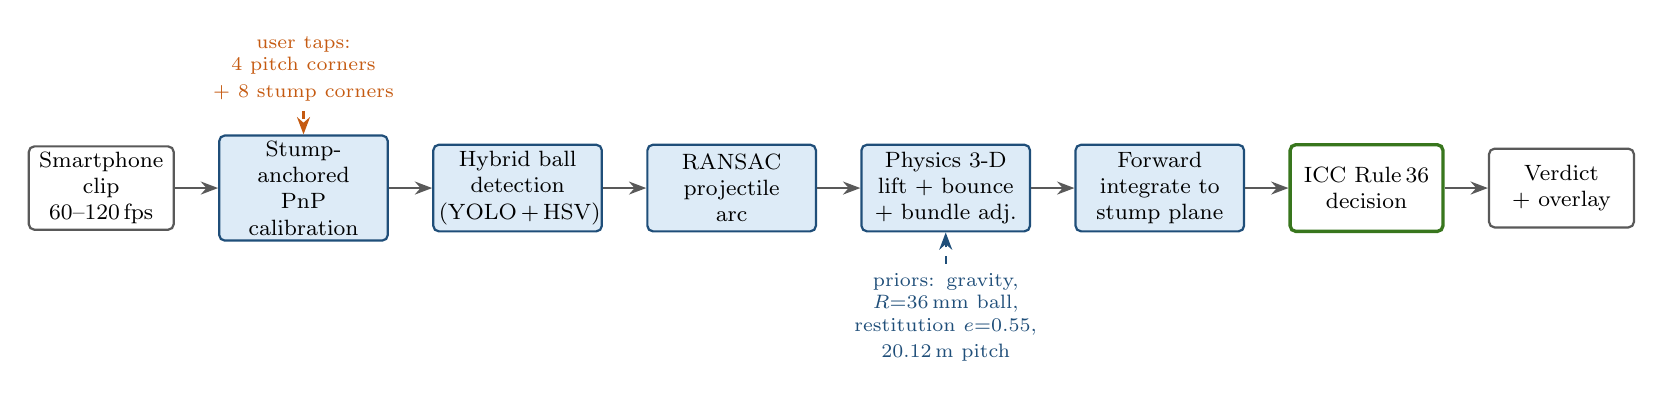
\begin{tikzpicture}[
  font=\footnotesize,
  node distance=6.5mm and 5.5mm,
  block/.style={rectangle, rounded corners=2pt, draw=pdblue, thick,
    fill=pdlight, align=center, text width=20mm, minimum height=11mm,
    inner sep=2pt},
  io/.style={rectangle, rounded corners=2pt, draw=pdgray, thick,
    fill=white, align=center, text width=17mm, minimum height=10mm,
    inner sep=2pt},
  dec/.style={rectangle, rounded corners=2pt, draw=pdgreen, very thick,
    fill=white, align=center, text width=18mm, minimum height=11mm,
    inner sep=2pt},
  arr/.style={-{Stealth[length=2.2mm]}, thick, draw=pdgray}
]
\node[io] (vid) {Smartphone\\clip\\60--120\,fps};
\node[block, right=of vid] (cal) {Stump-anchored\\PnP\\calibration};
\node[block, right=of cal] (det) {Hybrid ball\\detection\\(YOLO\,+\,HSV)};
\node[block, right=of det] (ran) {RANSAC\\projectile\\arc};
\node[block, right=of ran] (rec) {Physics 3-D\\lift + bounce\\+ bundle adj.};
\node[block, right=of rec] (pred) {Forward\\integrate to\\stump plane};
\node[dec, right=of pred] (lbw) {ICC Rule\,36\\decision};
\node[io, right=of lbw] (out) {Verdict\\+ overlay};

\draw[arr] (vid) -- (cal);
\draw[arr] (cal) -- (det);
\draw[arr] (det) -- (ran);
\draw[arr] (ran) -- (rec);
\draw[arr] (rec) -- (pred);
\draw[arr] (pred) -- (lbw);
\draw[arr] (lbw) -- (out);

% annotation of user taps into calibration
\node[align=center, text=pdaccent, above=3mm of cal, text width=24mm]
  (taps) {\scriptsize user taps:\\4 pitch corners\\+ 8 stump corners};
\draw[arr, draw=pdaccent, dashed] (taps) -- (cal);

% priors into reconstruction
\node[align=center, text=pdblue, below=4mm of rec, text width=30mm]
  (prior) {\scriptsize priors: gravity, $R{=}36$\,mm ball,\\restitution $e{=}0.55$,\\20.12\,m pitch};
\draw[arr, draw=pdblue, dashed] (prior) -- (rec);
\end{tikzpicture}%
}
\caption{PocketDRS processing pipeline. A single portrait clip and a small set
of user taps on the pitch corners and the two stump sets drive a stump-anchored
PnP calibration. A hybrid detector and a RANSAC projectile filter isolate the
ball's 2-D arc, which is lifted to metric 3-D under physical priors (gravity, a
known-radius ball, a single restitution-governed bounce, and the regulation
pitch length) and refined by bundle adjustment. The post-bounce trajectory is
forward-integrated to the stump plane and adjudicated under ICC Rule~36.}
\label{fig:pipeline}
\end{figure*}

\paragraph*{World frame} We adopt a right-handed pitch frame with origin at the
striker's stumps: $X$ runs down the pitch toward the bowler's end, $Y$ is
lateral (across the pitch), and $Z$ is vertical. The regulation pitch length
$L=20.12$\,m and stump height $h_s=0.711$\,m provide the metric scale.

Table~\ref{tab:compare} contrasts PocketDRS with a conventional multi-camera
DRS. The comparison is deliberately unflattering on accuracy: a single view
cannot triangulate, and our system's estimates of any depth-dependent quantity
are correspondingly weaker. What the table is meant to convey is a difference in
\emph{operating point}---a broadcast DRS optimizes officiating-grade accuracy at
high cost and fixed installation, whereas PocketDRS optimizes accessibility and
zero marginal cost at review-not-officiate accuracy.

\begin{table}[!t]
\caption{Operating point: multi-camera broadcast DRS versus PocketDRS.}
\label{tab:compare}
\centering
\footnotesize
\renewcommand{\arraystretch}{1.3}
\setlength{\tabcolsep}{3.5pt}
\begin{tabular}{@{}p{2.5cm}p{2.4cm}p{2.6cm}@{}}
\toprule
& \textbf{Multi-camera DRS} & \textbf{PocketDRS}\\
\midrule
Cameras & 6--8 calibrated high-speed & 1 commodity phone\\
Depth cue & triangulation (wide baselines) & physical priors + apparent size\\
Rig / install & fixed, per-ground & none\\
Calibration & surveyed, professional & user taps on stumps/pitch\\
Marginal cost & high & zero\\
Accuracy regime & officiating-grade & review / indicative\\
Intended use & match adjudication & coaching, training, education\\
\bottomrule
\end{tabular}
\end{table}

\section{Method}
\label{sec:method}

\subsection{Camera model and stump-anchored calibration}
\label{sec:calib}

We use a pinhole camera with intrinsics
\begin{equation}
\mathbf{K}=\begin{bmatrix} f_x & 0 & c_x\\ 0 & f_y & c_y\\ 0 & 0 & 1\end{bmatrix},
\end{equation}
assuming square pixels ($f_x=f_y$) and principal point at the image centre,
which is a good approximation for modern phone main cameras. A world point
$\mathbf{X}=(X,Y,Z)^\top$ projects to pixel $(u,v)$ via
\begin{equation}
s\begin{bmatrix}u\\v\\1\end{bmatrix}
=\mathbf{K}\,[\mathbf{R}\mid\mathbf{t}]\begin{bmatrix}\mathbf{X}\\1\end{bmatrix},
\quad
u=f_x\frac{X_c}{Z_c}+c_x,\;\; v=f_y\frac{Y_c}{Z_c}+c_y,
\label{eq:proj}
\end{equation}
where $(X_c,Y_c,Z_c)^\top=\mathbf{R}\mathbf{X}+\mathbf{t}$ is the point in
camera coordinates and $Z_c$ is its depth. An initial focal length is seeded
from an assumed horizontal field of view $\theta$ (default $67^\circ$),
\begin{equation}
f_x=\frac{\ell_{\text{px}}/2}{\tan(\theta/2)},
\label{eq:focal}
\end{equation}
with $\ell_{\text{px}}$ the number of pixels along the sensor's wide axis (the
image's long axis, which for portrait clips is the image height). This seed is
only a starting point; the calibration below refines it.

Rather than assume the lens is calibrated, we anchor on the two things whose
metric geometry is guaranteed by the Laws: the pitch rectangle and the two sets
of stumps. The user taps the four pitch corners and the eight outer corners of
the striker- and bowler-end stump sets. Each stump set is modelled as a planar
rectangle of half-width $w_{o}=0.132$\,m (the outer stump offset
$0.114$\,m plus the stump half-thickness $0.018$\,m) and height $h_s=0.711$\,m,
placed at $X=0$ (striker) and $X=L$ (bowler); the pitch corners lie at
$(0,\pm w_p,0)$ and $(L,\pm w_p,0)$ with $w_p$ the half pitch-width. Given these
2-D/3-D correspondences we solve for the pose $(\mathbf{R},\mathbf{t})$ by
minimizing reprojection error,
\begin{equation}
(\mathbf{R}^\star,\mathbf{t}^\star)=\arg\min_{\mathbf{R},\mathbf{t}}
\sum_{i}\bigl\lVert \pi(\mathbf{K};\mathbf{R},\mathbf{t};\mathbf{X}_i)-\mathbf{x}_i\bigr\rVert^2,
\label{eq:pnp}
\end{equation}
where $\pi(\cdot)$ is the projection~\eqref{eq:proj}. Because the seed focal
length~\eqref{eq:focal} and the pitch length may be imperfect, the solver
\emph{sweeps} over a range of field-of-view values (and, when unpinned, pitch
length) and keeps the pose with the lowest root-mean-square (RMS) reprojection
error $\varepsilon=\sqrt{\frac1N\sum_i\lVert\cdot\rVert^2}$. The stumps, whose
$0.711$\,m height is exact, carry the metric scale; the pitch corners are folded
into the joint solve only when they do not inflate the joint reprojection error
beyond a frame-scaled tolerance ($\max(6,\,0.012\,W)$ pixels at width $W$),
otherwise a stumps-only solution is trusted. In production the pitch length is
pinned to the regulation $20.12$\,m; the unpinned auto-fit is retained for
non-regulation surfaces. Finally, the camera \emph{end} (behind the bowler
versus behind the striker) is inferred from which stump rectangle subtends the
larger image area---the near end---which in turn fixes the sign convention used
by the decision layer.

\subsection{Ball detection}
\label{sec:detect}

Detection produces, per frame, a set of candidate balls with pixel centre
$(u,v)$, pixel radius $r$, and a confidence weight. Two detectors run:
\begin{itemize}
\item a \emph{learned} detector---a custom-trained Ultralytics YOLO model
(\emph{cricket\_ball.pt})---which is robust to the moving people and net
clutter that dominate real footage; and
\item a \emph{classical} detector combining HSV colour thresholding (by ball
hue) with frame-difference motion blobs, which needs no weights and is effective
on clean, high-contrast clips.
\end{itemize}
An automatic selector prefers the learned track. A candidate track is scored by
how well it forms a single long, smooth projectile arc rather than a
large-span clutter track (e.g.\ a bowler's diagonal run-up). The colour track
\emph{overrides} the learned track only when it is both markedly longer
\emph{and} an absolutely tight projectile arc in an absolute sense---not merely
looser than YOLO---because on near end-on views a clutter track can sit only
slightly looser than the true ball yet be geometric nonsense. This guards
against locking onto the run-up or onto a second moving object.

\subsection{Robust 2-D arc extraction}
The retained detections still include points from before release and after bat
impact. A two-pass RANSAC~\cite{fischler1981ransac} projectile fit over the
per-frame detections keeps, as its inlier set, the largest subset consistent
with a single smooth image-space parabola:
\begin{equation}
\text{maximize}\;\bigl|\{i: \operatorname{res}_i(\hat{\mathbf p})<\tau\}\bigr|
\quad\text{over minimal samples of }\hat{\mathbf p},
\end{equation}
with $\operatorname{res}_i$ the geometric residual to the fitted arc and $\tau$
a pixel tolerance. This isolates one clean delivery and rejects sideways
excursions into adjacent nets.

\subsection{Physics-constrained 3-D reconstruction}
\label{sec:recon}

The 2-D inlier arc is lifted to a metric 3-D trajectory. The core cue that
breaks the depth ambiguity of a single view, in addition to the projectile
constraint, is the ball's known physical radius $R=0.036$\,m. A sphere of radius
$R$ at depth $d$ subtends an apparent pixel radius
\begin{equation}
r=\frac{f_x R}{d}\quad\Longrightarrow\quad d=\frac{f_x R}{r},
\label{eq:depthsize}
\end{equation}
so the detected radius seeds a per-point depth and thus metric scale. Because
$d\propto 1/r$, this cue is precise only when the ball is large in the image
(near the camera) and degrades rapidly with distance; we therefore use it as a
seed and a weak constraint, not as the primary estimate.

\paragraph*{Gravity-constrained linear solve} Following the projectile-prior
approach of~\cite{ribnick2009projectiles}, we first obtain a world trajectory by
a linear least-squares solve that enforces constant horizontal velocity and
constant vertical acceleration $-g$ ($g=9.81\,\mathrm{m/s^2}$):
\begin{align}
X(t)&=X_0+v_x t, & Y(t)&=Y_0+v_y t,\notag\\
Z(t)&=Z_0+v_z t-\tfrac{1}{2}g\,t^2.
\label{eq:proj_motion}
\end{align}
Depth along the optical axis is scaled by the correct ray geometry for off-axis
points, so that a ball moving away from an obliquely placed camera is not
foreshortened incorrectly.

\paragraph*{Single restitution-governed bounce} A delivery that pitches has one
ground contact. We search the middle $60\%$ of the observed time span for a
split time $t_b$ that best partitions the detections into a pre- and a
post-bounce parabola, accepting the bounce only if it reduces the fit RMS by at
least $10\%$. At the bounce the vertical velocity reverses and loses energy with
coefficient of restitution $e=0.55$,
\begin{equation}
v_z^{+}=-\,e\,\bigl(v_z^{-}-g\,t_b\bigr),
\label{eq:restitution}
\end{equation}
where $v_z^{-}$ and $v_z^{+}$ are the vertical velocities immediately before and
after contact. Crucially, the horizontal post-bounce velocity is taken as the
\emph{measured} value from an independent fit to the post-bounce points whenever
that arc is well-determined (enough inliers, residual no worse than the
pre-bounce arc, and a physically plausible speed). This captures the seam/spin
deviation and the friction slow-down off the pitch that a pure restitution model
cannot; when the post-bounce arc is short or noisy, the pre-bounce velocity is
carried through instead. The vertical rebound always stays
restitution-derived~\eqref{eq:restitution}, which we found more stable than the
noisy measured vertical component.

\paragraph*{Bundle adjustment} The world trajectory is finally refined by
minimizing an image-space cost over the six trajectory parameters
$\Theta=(X_0,Y_0,Z_0,v_x,v_y,v_z)$ using a trust-region least-squares
solver~\cite{more1978lm,virtanen2020scipy}:
\begin{equation}
\min_{\Theta}\sum_i \Bigl[(u_i-\hat u_i)^2+(v_i-\hat v_i)^2
+\lambda\Bigl(\tfrac{r_i}{\hat r_i}-1\Bigr)^2\Bigr]+\Omega(\Theta),
\label{eq:ba}
\end{equation}
where $(\hat u_i,\hat v_i)$ and $\hat r_i=f_xR/\hat d_i$ are the reprojected
centre and radius of the model point at time $t_i$ via~\eqref{eq:proj}
and~\eqref{eq:depthsize}. Pixel-centre residuals dominate; the multiplicative
radius residual is down-weighted ($\lambda$ small, and further weighted toward
larger, more reliable detections) because it is informative only at close
range. A soft prior $\Omega(\Theta)$ nudges the trajectory to span most of the
pitch, which is essential when the ball travels nearly along the optical axis
and depth-from-size alone cannot localize it longitudinally. If a bounce was
found, it is kept as a fixed knot and only the pre-bounce parameters are
refined, with the post-bounce arc determined by joint continuity.

\subsection{Depth-error sensitivity}
\label{sec:sensitivity}
It is worth making explicit, from the model itself, why depth-coupled quantities
are the weak link. Differentiating the depth-from-size
relation~\eqref{eq:depthsize} with respect to the measured pixel radius gives
\begin{equation}
\frac{\partial d}{\partial r}=-\frac{f_x R}{r^2}=-\frac{d}{r},
\qquad\Rightarrow\qquad
\frac{\delta d}{d}=\frac{\delta r}{r}.
\label{eq:sens_rel}
\end{equation}
The relative depth error equals the relative radius error. Substituting
$r=f_xR/d$ converts this into an \emph{absolute} depth error that grows
quadratically with distance for a fixed radius-measurement noise $\delta r$:
\begin{equation}
\delta d=\frac{d}{r}\,\delta r=\frac{d^2}{f_x R}\,\delta r.
\label{eq:sens_abs}
\end{equation}
A ball twice as far away therefore incurs roughly four times the depth error
from the same sub-pixel detection noise. Because the bounce, the impact, and
the release all occur down the pitch---far from a camera behind either
batter---their longitudinal (depth) coordinates, and the release speed derived
by differencing them, inherit this amplification. The lateral coordinate at the
stumps, by contrast, is fixed by the calibrated stump \emph{projection}
in~\eqref{eq:proj} rather than by apparent size, and so is not subject
to~\eqref{eq:sens_abs}; this is the analytical reason the lateral stump-plane
error is two orders of magnitude smaller than the depth error in
Section~\ref{sec:results}. Equation~\eqref{eq:sens_abs} also motivates our design
choices: seeding rather than trusting depth-from-size, adding the gravity and
pitch-traversal priors that supply the missing longitudinal information, and
widening the vertical umpire's-call band.

\subsection{Prediction to the stump plane}
The post-bounce projectile~\eqref{eq:proj_motion} is forward-integrated to the
striker's stump plane $X=0$, giving the predicted lateral and vertical impact
point $(y^\star,z^\star)$ where the ball would cross the stumps.

\subsection{LBW decision}
\label{sec:lbw}

The decision implements the three ICC Rule~36 tests~\cite{mcc2017laws}:
pitching in line, impact in line, and wickets hitting. Off and leg sides are
resolved from a signed convention $\sigma\in\{+1,-1\}$ derived from the batter's
handedness \emph{and} the inferred camera end (Section~\ref{sec:calib}); a
left-handed batter flips the sign, and a behind-the-bowler view mirrors it
relative to a behind-the-striker view.

\emph{Pitching in line.} If the bounce point lies more than one stump-width
outside the leg stump ($y_b\,\sigma > w_{\text{half}}+0.1143$\,m, with
$w_{\text{half}}=0.1143$\,m the half stump width), the ball pitched outside leg
and the batter cannot be out; the check fails.

\emph{Impact in line.} Impact outside the leg stump ($y_i\,\sigma>0$ beyond the
line) is always not out.

\emph{Wickets hitting.} The ball is projected to hit the stumps when
\begin{equation}
|y^\star|\le w_g \;\;\text{and}\;\; 0\le z^\star\le h_s+R,
\end{equation}
with the lateral wicket guard $w_g=w_{\text{half}}+R=0.150$\,m (the outer stump
edge plus a ball radius) and the top guard the bail height plus a ball radius.

\emph{Umpire's-call bands.} A monocular system resolves the vertical/depth axis
less well than the lateral axis. We therefore apply anisotropic umpire's-call
margins: a marginal clip becomes \textsc{umpire's call} when the predicted path
grazes the stump boundary within $m_y=R=3.6$\,cm laterally or $m_z=2R=7.2$\,cm
vertically---the vertical band is deliberately twice the lateral one. The
tightest axis decides. A symmetric $5$\,cm band on the \emph{outside} of the
stumps flags a ``just missing'' path only when the ball had first passed the
pitching and impact tests. Algorithm~\ref{alg:lbw} summarizes the decision.

\begin{algorithm}[!t]
\caption{ICC Rule~36 decision with monocular bands}
\label{alg:lbw}
\begin{algorithmic}[1]
\REQUIRE bounce $y_b$, impact $y_i$, predicted stump point $(y^\star,z^\star)$,
sign $\sigma$
\STATE $\text{checks}\gets\{\textsc{pitch},\textsc{impact}\}=\textsc{true},\ \textsc{hit}=\textsc{false}$
\IF{$y_b\,\sigma>w_{\text{half}}+0.1143$}
  \STATE $\textsc{pitch}\gets\textsc{false}$ \COMMENT{pitched outside leg}
\ENDIF
\IF{$y_i\,\sigma>$ leg line}
  \STATE $\textsc{impact}\gets\textsc{false}$ \COMMENT{impact outside leg}
\ENDIF
\IF{$|y^\star|\le w_g$ \AND $0\le z^\star\le h_s+R$}
  \STATE $\textsc{hit}\gets\textsc{true}$
  \STATE $m\gets\min(w_g-|y^\star|,\ (h_s+R)-z^\star)$
  \IF{$w_g-|y^\star|\le m_y$ \OR $(h_s+R)-z^\star\le m_z$}
    \STATE \textbf{return} \textsc{umpire's call}
  \ENDIF
\ENDIF
\IF{$\textsc{pitch}\wedge\textsc{impact}\wedge\textsc{hit}$}
  \STATE \textbf{return} \textsc{out}
\ELSIF{$\textsc{pitch}\wedge\textsc{impact}$ \AND path within $5$\,cm outside stumps}
  \STATE \textbf{return} \textsc{umpire's call}
\ELSE
  \STATE \textbf{return} \textsc{not out}
\ENDIF
\end{algorithmic}
\end{algorithm}

\section{Experimental Setup}
\label{sec:setup}

We evaluate PocketDRS along three axes: (i) a synthetic harness with exact
ground truth, (ii) real hand-held net clips, and (iii) a generalization probe on
unseen internet footage. The synthetic harness is the only setting in which a
metric ground-truth trajectory is available, so it carries the quantitative
accuracy claims; the real clips test the end-to-end system on genuine sensor
noise, motion blur, and clutter.

\paragraph*{Implementation} The pipeline is implemented as an offline
server-side job in Python, using OpenCV~\cite{bradski2000opencv} for image
processing and geometry, the Ultralytics YOLO
runtime~\cite{jocher2023ultralytics} for learned detection, and SciPy's
trust-region least-squares solver~\cite{virtanen2020scipy} for the bundle
adjustment~\eqref{eq:ba} and the projectile fits. A job takes the raw clip, the
frame rate, the user annotations, and the batter handedness, and returns the
verdict, the three ICC checks, the reconstructed metric trajectory, and a
rendered overlay video. Processing is per-clip and non-interactive, which suits
the coaching use case (review after the session) rather than live officiating.

\paragraph*{Synthetic harness} We render eight deliveries with known physics: a
release speed of $115$\,km/h, three line families (off, middle, leg), lengths of
approximately $5.5$--$6.0$\,m, at $60$\,frames/s, with the virtual camera placed
behind the striker. Because the generating trajectory is known exactly, we can
measure absolute errors in the reconstructed bounce point, impact point,
predicted stump-plane crossing, and release speed, and compare the predicted LBW
verdict against the ground-truth verdict.

\paragraph*{Real clips} We captured single-phone net clips spanning the
conditions a grassroots user would encounter: outdoor and indoor nets, red and
white balls, off- and leg-spin, and both camera ends. Each was tracked
end-to-end and rendered with a broadcast-style overlay
(Fig.~\ref{fig:overlay}). Here we report the recovered speed, the verdict and
its cause, and the calibration reprojection error as an internal quality metric;
no metric ground truth is available for these clips.

\paragraph*{Generalization probe} To probe behaviour on truly unseen footage we
ran the learned detector and tracker on four arbitrary net-practice clips from
public video, testing both whether the detector locks onto the real ball and
whether the system \emph{declines} clips that violate its assumptions.

\section{Results}
\label{sec:results}

\subsection{Synthetic ground-truth accuracy}
Table~\ref{tab:synth} reports the synthetic results. PocketDRS reproduced the
ground-truth LBW verdict in $\mathbf{8/8}$ deliveries. The predicted ball
position at the stump plane---the quantity the LBW verdict actually depends
on---had a mean error of $11.7$\,cm and a maximum of $21.4$\,cm. This error is
strongly anisotropic: the lateral ($y$) component averaged just $0.3$\,cm, while
the vertical ($z$) component averaged $11.7$\,cm and accounts for essentially
all of the total. This is the expected signature of monocular reconstruction:
the lateral position, well constrained by the calibrated stump geometry, is
recovered accurately, whereas the vertical/depth-coupled component, which
depends on the weak depth-from-size cue, is not.

\begin{table}[!t]
\caption{Synthetic ground-truth validation (8 deliveries, 115\,km/h, 60\,fps,
camera behind striker).}
\label{tab:synth}
\centering
\renewcommand{\arraystretch}{1.25}
\begin{tabular}{@{}lr@{}}
\toprule
\textbf{Metric} & \textbf{Value}\\
\midrule
LBW verdict agreement with ground truth & $8/8$ ($100\%$)\\
Predicted stump-plane position error (mean) & $11.7$\,cm\\
\quad --- maximum & $21.4$\,cm\\
\quad --- lateral $y$ component (mean) & $0.3$\,cm\\
\quad --- vertical $z$ component (mean) & $11.7$\,cm\\
Bounce-point error (mean) & $54.7$\,cm\\
Impact-point error (mean) & $48.8$\,cm\\
Release-speed error (mean) & $22.1$\,km/h\\
\bottomrule
\end{tabular}
\end{table}

The bounce-point ($54.7$\,cm mean) and impact-point ($48.8$\,cm mean) errors are
much larger, and the release-speed error ($22.1$\,km/h mean) is large enough
that we report absolute speed only as an \emph{indicative} figure. On a
near-axial monocular view the down-pitch (depth) position is the least
observable coordinate, so both the longitudinal location of the bounce and the
time-derivative that yields speed are poorly constrained. It is notable, and
central to why the system is nonetheless useful for LBW, that the verdict-
critical stump-plane crossing is an order of magnitude better resolved than
these intermediate quantities: the geometry that matters for LBW (lateral line
and height at the stumps) is precisely the geometry the stump-anchored
calibration constrains best.

\subsection{Real hand-held clips}
Table~\ref{tab:real} summarizes three representative single-phone clips. All
were tracked end-to-end and produced a coherent verdict with a plausible
recovered speed. The calibration reprojection error---an internal consistency
metric---ranged from $2.1$ to $10.6$\,px; the largest value ($10.6$\,px, the
outdoor white-ball clip) is consistent with a harder detection and marking
setting yet still yielded a stable pose and a sensible \textsc{not out} call.
The recovered spin-bowling speeds ($38$--$84$\,km/h) are in the correct regime,
though, per the synthetic analysis, absolute speed should be read with caution.

\begin{table}[!t]
\caption{Real single-phone net clips (end-to-end, overlay rendered). Reproj.\ is
the calibration RMS reprojection error.}
\label{tab:real}
\centering
\footnotesize
\renewcommand{\arraystretch}{1.25}
\setlength{\tabcolsep}{4pt}
\begin{tabular}{@{}lcccc@{}}
\toprule
\textbf{Clip} & \textbf{Setting} & \textbf{Speed} & \textbf{Verdict} & \textbf{Reproj.}\\
\midrule
test3 & outdoor, white, off-spin & $84$\,km/h & \textsc{not out}$^{a}$ & $10.6$\,px\\
test4 & indoor, red, leg-spin & $58$\,km/h & \textsc{not out}$^{b}$ & $3.7$\,px\\
test5 & indoor, red, off-spin & $38$\,km/h & \textsc{not out}$^{c}$ & $2.1$\,px\\
\bottomrule
\end{tabular}
\\[2pt]
\raggedright\scriptsize
$^{a}$predicted path misses the stumps;\;
$^{b}$pitched and impact outside the leg line;\;
$^{c}$near end-on, predicted path wide of the stumps.
\end{table}

\begin{figure}[!t]
\centering
\IfFileExists{../validation/test4/test4_sample.png}{%
  \begin{subfigure}{\columnwidth}
    \centering
    \includegraphics[width=\columnwidth,height=0.42\columnwidth,keepaspectratio]%
      {../validation/test4/test4_sample.png}
    \caption{Broadcast-style tracking overlay on a real clip.}
  \end{subfigure}\\[4pt]
  \IfFileExists{../validation/test4/test4_3d.png}{%
    \begin{subfigure}{\columnwidth}
      \centering
      \includegraphics[width=\columnwidth,height=0.42\columnwidth,keepaspectratio]%
        {../validation/test4/test4_3d.png}
      \caption{Reconstructed 3-D trajectory and predicted stump-plane crossing.}
    \end{subfigure}}{}%
}{%
  \fbox{\parbox[c][0.5\columnwidth][c]{0.9\columnwidth}{\centering\itshape
  (Overlay and 3-D reconstruction figures are generated by the pipeline for each
  clip; image assets omitted from this build.)}}%
}
\caption{Qualitative output on the indoor red-ball leg-spin clip (test4). The
overlay shows the tracked 2-D arc; the 3-D view shows the reconstructed metric
trajectory forward-integrated to the stump plane, which here pitches and impacts
outside the leg line, giving \textsc{not out}.}
\label{fig:overlay}
\end{figure}

\subsection{Generalization to unseen footage}
On four arbitrary internet net clips, the learned detector locked onto and
tracked the real ball in $3$ of $4$, yielding $12$--$24$ inlier points per
delivery---sufficient for a projectile fit. A full 3-D LBW review, however,
requires both stump sets to be cleanly visible for the stump-anchored
calibration and a rectilinear (non-fisheye) lens. The system correctly
\emph{declined} the two clips that violated these preconditions---a wide
fisheye clip and a clip in which the batter occluded a stump set---rather than
emitting a fabricated verdict. We regard this as the desired behaviour: the
value of a review system lies as much in knowing when \emph{not} to rule as in
ruling.

\section{Discussion and Limitations}
\label{sec:discussion}

\paragraph*{Monocular depth is the dominant error} The synthetic results make
the central limitation quantitative: lateral position at the stumps is accurate
($0.3$\,cm mean) but the vertical/depth-coupled component ($11.7$\,cm mean) is
an order of magnitude worse, and intermediate depth-dependent quantities
(bounce, impact, speed) are worse still. This is intrinsic to single-view
geometry and cannot be removed by better software alone; it is the reason a
monocular system must never be presented as equivalent to multi-camera
triangulation. Our design responds to this by (i) anchoring on lateral stump
geometry, which is well observed, (ii) constraining depth with physical priors,
and (iii) widening the vertical umpire's-call band to $2R$ so that marginal
height calls are surfaced as reviews rather than asserted.

\paragraph*{Absolute speed is unreliable} With a mean release-speed error of
$22.1$\,km/h on a near-axial view, PocketDRS should be understood to report
speed as a rough indicator, not a measurement. Speed along the optical axis is
exactly the coordinate the geometry constrains least.

\paragraph*{Calibration dependence} The metric scale rests entirely on the
user's taps on the stump corners and on both stump sets being visible and
rectilinearly imaged. Poor taps, a fisheye lens, or an occluded stump set
degrade or preclude the solve; the reprojection error is exposed precisely so
that a bad calibration is visible rather than silent.

\paragraph*{Single-view assumptions} The bounce model assumes one ground
contact and a fixed vertical restitution; the horizontal deviation is measured
but only when the post-bounce arc is well sampled. Deliveries with unusual
bounce, double contact, or very short post-bounce visibility fall back to weaker
estimates. The system is not ICC-certified and makes no claim to officiating
accuracy.

\paragraph*{Threats to validity} The quantitative accuracy figures come from a
synthetic harness, so they inherit its idealizations: a noise-free renderer, a
single release speed ($115$\,km/h), a camera behind the striker, and eight
deliveries. Real sensor noise, rolling-shutter distortion, motion blur, and
frame-rate jitter will widen the errors, and the sample is too small to place
tight confidence intervals on the means. The real-clip evaluation exercises
those nuisance factors but lacks metric ground truth, so it can only confirm
end-to-end coherence, not accuracy. We have been careful to separate these two
kinds of evidence throughout and to draw the numerical claims only from the
setting in which ground truth exists.

\paragraph*{Where it is useful} Despite these limits the verdict-critical
quantity---the lateral line and height at the stumps---is well enough resolved
to agree with ground truth on all synthetic cases and to produce coherent,
explainable calls on real footage. The realistic deployment is therefore
coaching and training: giving a bowler or batter at club, school, or age-group
level an objective, repeatable second opinion and an educational visualization
of ball flight, at zero hardware cost, rather than replacing an on-field umpire.

\section{Conclusion and Future Work}
\label{sec:conclusion}

We presented PocketDRS, a single-smartphone LBW review system that replaces the
missing viewpoints of multi-camera DRS with cricket-specific physical priors: a
stump-anchored PnP calibration, a hybrid clutter-aware detector, a RANSAC
projectile filter, and a physics-constrained monocular 3-D lift with a
restitution-governed bounce and image-space bundle adjustment, adjudicated under
ICC Rule~36 with anisotropic umpire's-call bands. On synthetic ground truth it
agrees with the true verdict on all eight deliveries and predicts the
stump-plane crossing to $11.7$\,cm on average, while being candidly weak on
absolute depth-dependent quantities such as bounce location and release speed.

Future work targets the depth weakness directly. The most direct improvement is
a second viewpoint---a stereo pair or two synchronized phones---which would
restore true triangulation for the vertical/depth axis while preserving the
rig-free ethos. Learned monocular depth priors could strengthen the
depth-from-size cue, and automatic stump and crease detection would remove the
manual tapping that currently gates both accuracy and generalization. We also
plan a larger real-clip study with instrumented ground truth to place
confidence intervals on the field estimates rather than the synthetic ones
alone.

\section*{Acknowledgment}
The author thanks the project supervisors at Phoenix College of Management
(Lincoln University) for their guidance.

\begin{thebibliography}{99}

\bibitem{zhang2000calibration}
Z. Zhang, ``A flexible new technique for camera calibration,''
\emph{IEEE Trans. Pattern Anal. Mach. Intell.}, vol.~22, no.~11,
pp.~1330--1334, Nov. 2000.

\bibitem{hartley2004mvg}
R. Hartley and A. Zisserman, \emph{Multiple View Geometry in Computer Vision},
2nd~ed. Cambridge, U.K.: Cambridge Univ. Press, 2004.

\bibitem{ribnick2009projectiles}
E. Ribnick, S. Atev, and N. P. Papanikolopoulos, ``Estimating 3D positions and
velocities of projectiles from monocular views,''
\emph{IEEE Trans. Pattern Anal. Mach. Intell.}, vol.~31, no.~5, pp.~938--944,
May 2009.

\bibitem{fischler1981ransac}
M. A. Fischler and R. C. Bolles, ``Random sample consensus: A paradigm for model
fitting with applications to image analysis and automated cartography,''
\emph{Commun. ACM}, vol.~24, no.~6, pp.~381--395, Jun. 1981.

\bibitem{redmon2016yolo}
J. Redmon, S. Divvala, R. Girshick, and A. Farhadi, ``You only look once:
Unified, real-time object detection,'' in \emph{Proc. IEEE Conf. Comput. Vis.
Pattern Recognit. (CVPR)}, 2016, pp.~779--788.

\bibitem{jocher2023ultralytics}
G. Jocher, A. Chaurasia, and J. Qiu, ``Ultralytics YOLO,'' software, 2023.
[Online]. Available: \url{https://github.com/ultralytics/ultralytics}

\bibitem{huang2019tracknet}
Y.-C. Huang, I.-N. Liao, C.-H. Chen, T.-U. \.Ik, and W.-C. Peng, ``TrackNet: A
deep learning network for tracking high-speed and tiny objects in sports
applications,'' in \emph{Proc. IEEE Int. Conf. Adv. Video Signal-Based Surveill.
(AVSS)}, 2019, pp.~1--8.

\bibitem{owens2003hawkeye}
N. Owens, C. Harris, and C. Stennett, ``Hawk-eye tennis system,'' in
\emph{Proc. Int. Conf. Visual Information Engineering (VIE)}, 2003,
pp.~182--185.

\bibitem{thomas2017cvsports}
G. Thomas, R. Gade, T. B. Moeslund, P. Carr, and A. Hilton, ``Computer vision for
sports: Current applications and research topics,''
\emph{Comput. Vis. Image Underst.}, vol.~159, pp.~3--18, Jun. 2017.

\bibitem{bradski2000opencv}
G. Bradski, ``The OpenCV library,'' \emph{Dr. Dobb's Journal of Software Tools},
vol.~25, no.~11, pp.~120--125, 2000.

\bibitem{more1978lm}
J. J. Mor\'e, ``The Levenberg--Marquardt algorithm: Implementation and theory,''
in \emph{Numerical Analysis}, Lecture Notes in Mathematics, vol.~630. Berlin,
Germany: Springer, 1978, pp.~105--116.

\bibitem{virtanen2020scipy}
P. Virtanen \emph{et al.}, ``SciPy 1.0: Fundamental algorithms for scientific
computing in Python,'' \emph{Nature Methods}, vol.~17, pp.~261--272, 2020.

\bibitem{bailey2006cricket}
M. Bailey and S. R. Clarke, ``Predicting the match outcome in one day
international cricket matches, while the game is in progress,''
\emph{Journal of Sports Science and Medicine}, vol.~5, no.~4, pp.~480--487, 2006.

\bibitem{mcc2017laws}
Marylebone Cricket Club, \emph{The Laws of Cricket (2017 Code)}, Law~36
(Leg Before Wicket). London, U.K.: MCC, 2017.

\end{thebibliography}

\end{document}
